% \begin{center}
%     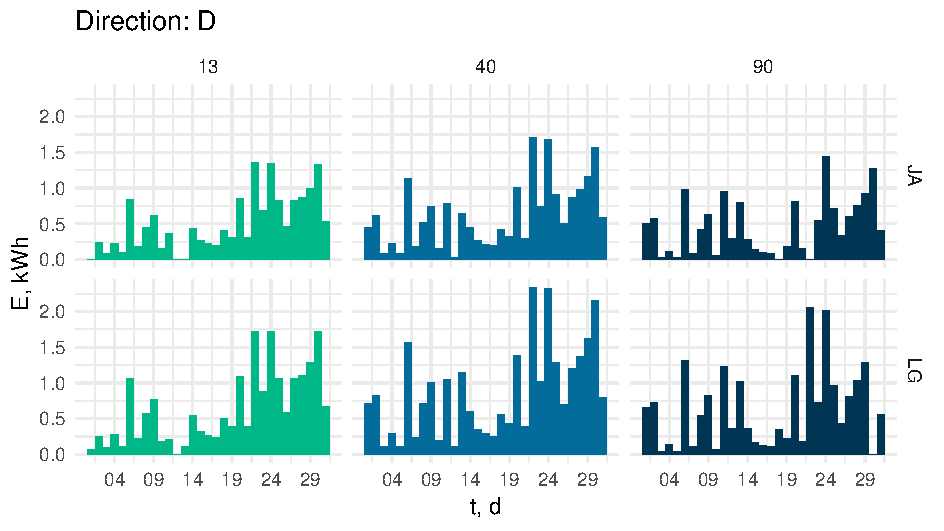
\includegraphics[width=\linewidth]{figures/mar_Degbar.pdf}
%     \captionof{figure}{Dienvidu saules paneļu saražotā enerģija dienā atkarībā no leņķa}
% \end{center}
% \begin{center}
%     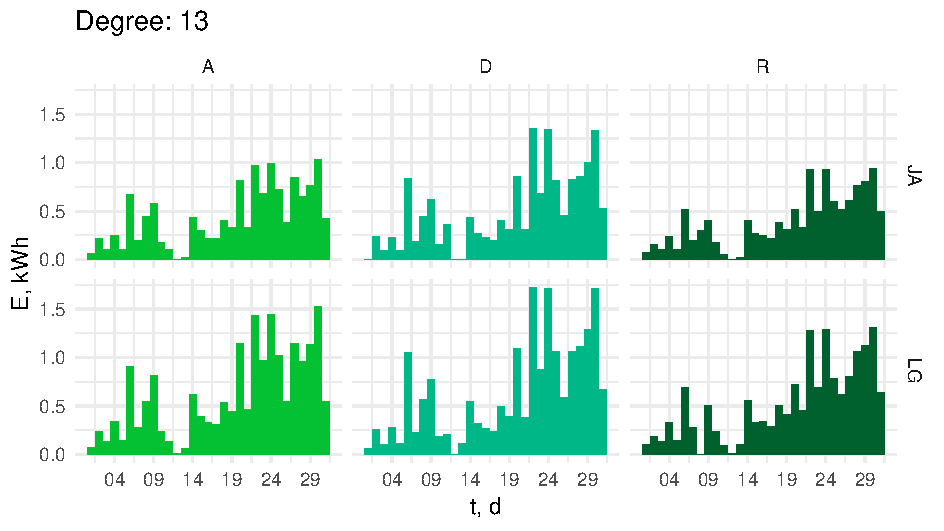
\includegraphics[width=\linewidth]{figures/mar_Dirbar.pdf}
%     \captionof{figure}{13 grādu leņķī esošo saules paneļu saražotā enerģija dienā atkarībā no debespuses}
% \end{center}
% \begin{center}
%     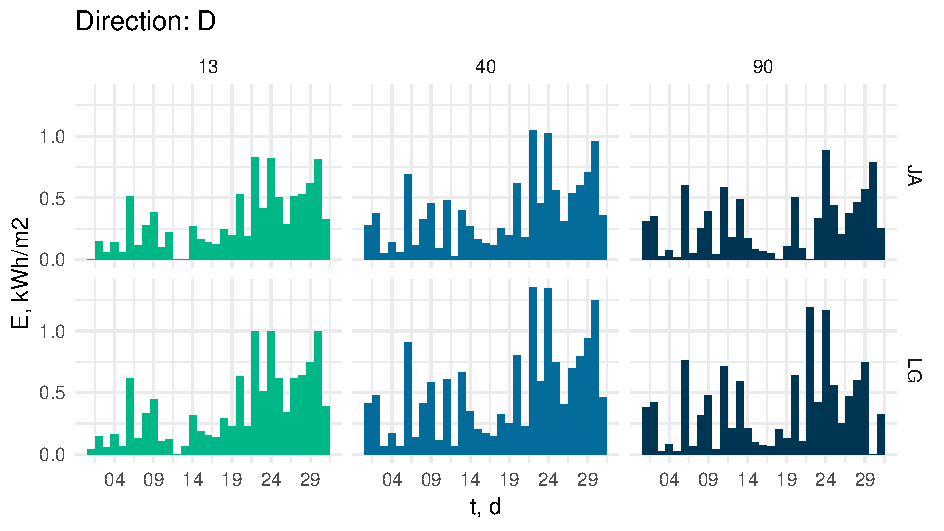
\includegraphics[width=\linewidth]{figures/mar_Degbarm2.pdf}
%     \captionof{figure}{Dienvidu saules paneļu saražotā enerģija dienā atkarībā no leņķa normēta uz saules paneļu laukumiem}
% \end{center}
% \begin{center}
%     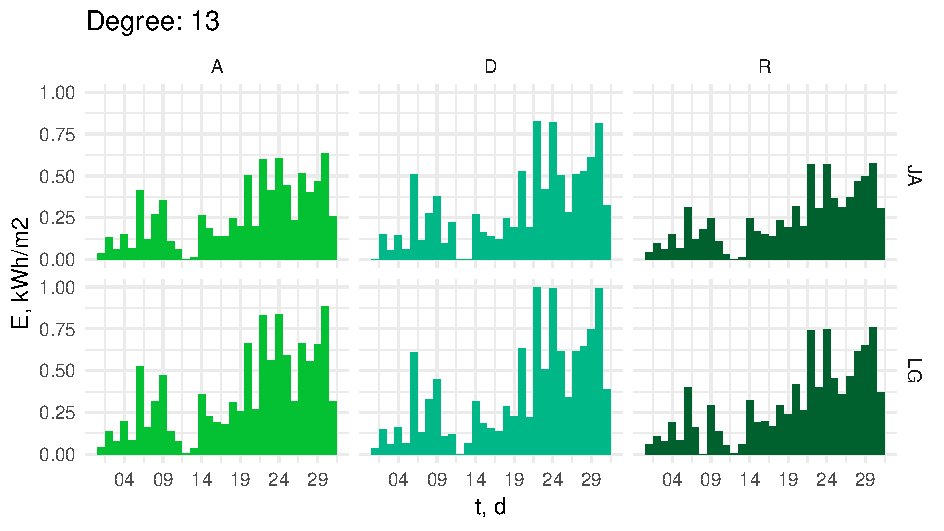
\includegraphics[width=\linewidth]{figures/mar_Dirbarm2.pdf}
%     \captionof{figure}{13 grādu leņķī esošo saules paneļu saražotā enerģija dienā atkarībā no leņķa normēta uz saules paneļu laukumiem}
% \end{center}
% \begin{center}
%     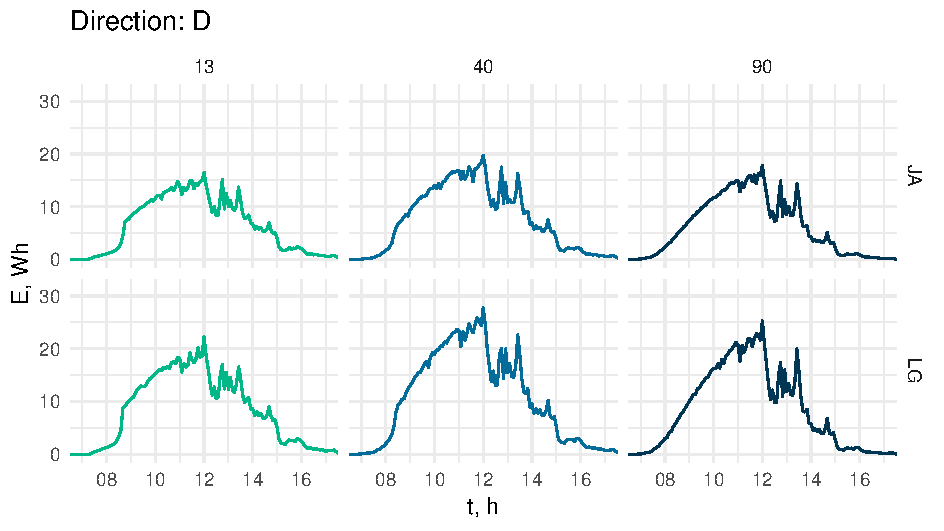
\includegraphics[width=\linewidth]{figures/mar_Deg_l.pdf}
%     \captionof{figure}{Tipisks saražotās enerģijas sadalījums dienā dienvidu saules paneļiem}
% \end{center}
% \begin{center}
%     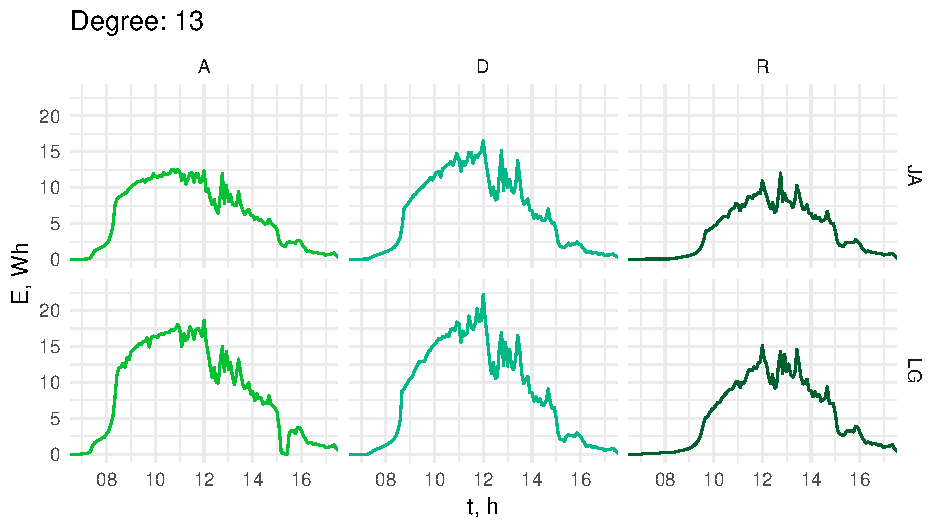
\includegraphics[width=\linewidth]{figures/mar_Dir_l.pdf}
%     \captionof{figure}{Tipisks saražotās enerģijas sadalījums dienā 13 grādu leņķī esošajiem saules paneļiem}
% \end{center}
% \begin{center}
%     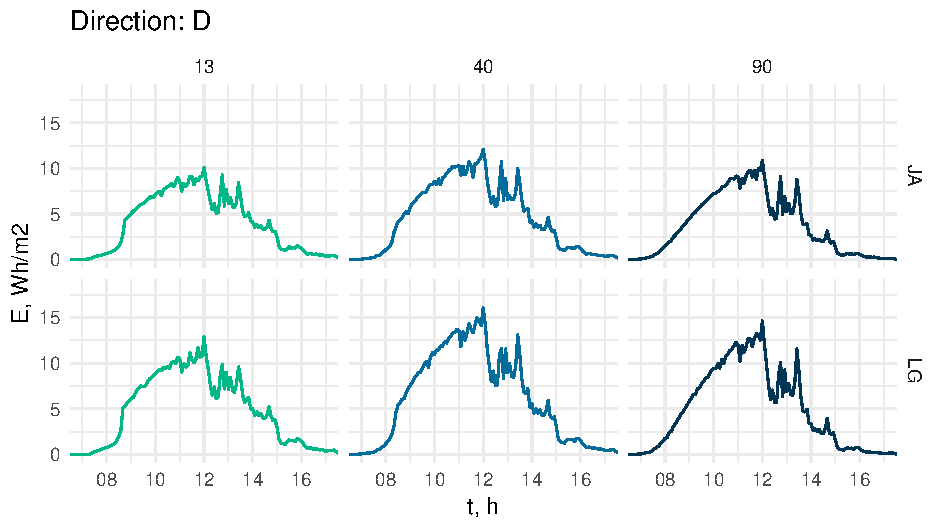
\includegraphics[width=\linewidth]{figures/mar_Deg_lm2.pdf}
%     \captionof{figure}{Tipisks saražotās enerģijas sadalījums dienā dienvidu saules paneļiem nrmēts uz saules paneļu laukumiem}
% \end{center}
% \begin{center}
%     \includegraphics[width=\linewidth]{figures/mar_Dir_m2.pdf}
%     \captionof{figure}{Tipisks saražotās enerģijas sadalījums dienā 13 grādu leņķī esošajiem saules paneļiem normēts uz saules paneļu laukumiem}
% \end{center}

% \begin{center}
%     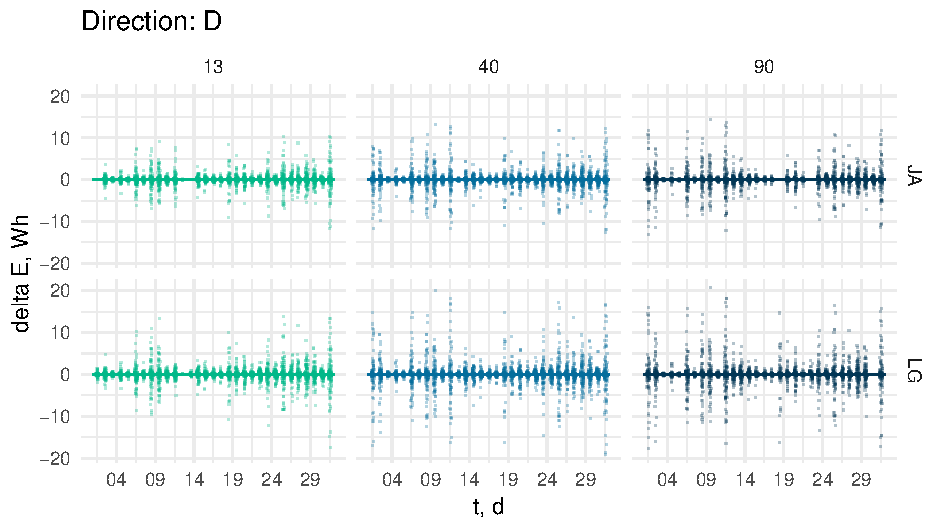
\includegraphics[width=\linewidth]{figures/mar_difDeg.pdf}
%     \captionof{figure}{Dienvidu saules paneļu enerģijas starpība dienā atkarībā no leņķa}
% \end{center}
% \begin{center}
%     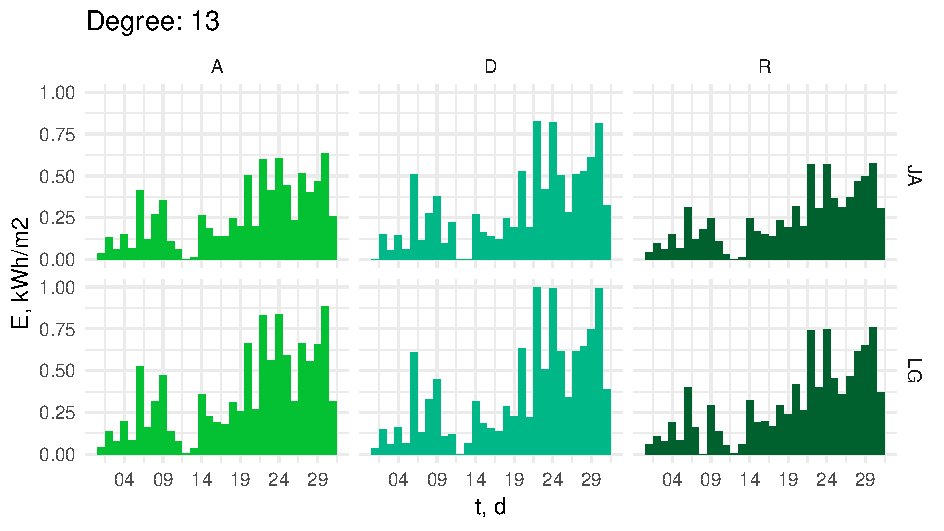
\includegraphics[width=\linewidth]{figures/mar_Dirbarm2.pdf}
%     \captionof{figure}{13 grādu leņķī esošo saules paneļu enerģijas starpība dienā atkarībā no debespuses}
% \end{center}

% \begin{center}
%     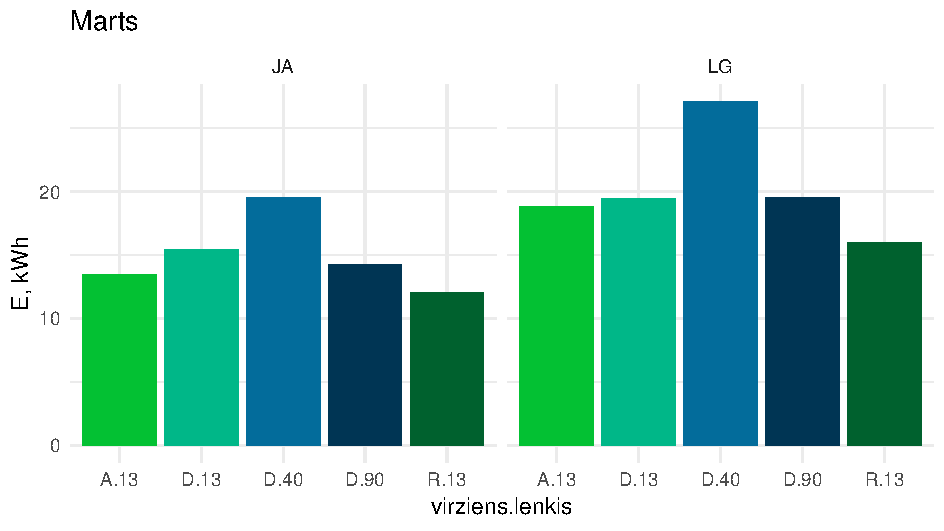
\includegraphics[width=\linewidth]{figures/mar_bar.pdf}
%     \captionof{figure}{Saules paneļu martā saražotā enerģija}
% \end{center}


% \begin{center}
%     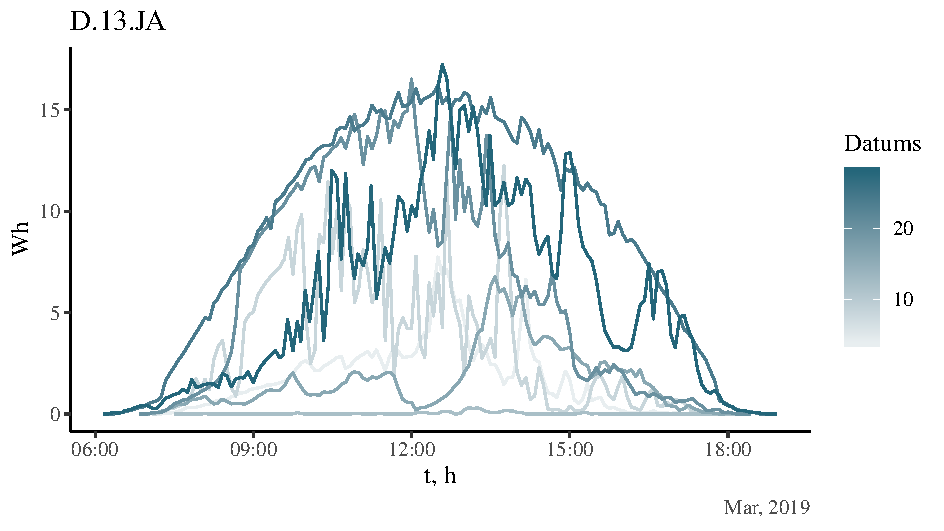
\includegraphics[width=\linewidth]{figures/mar_day/mar_D13JA.pdf}
%     \captionof{figure}{Saražotās enerģijas sadalījuma izmaiņas mēneša dienās saules panelim martā}
% \end{center}
% \begin{center}
%     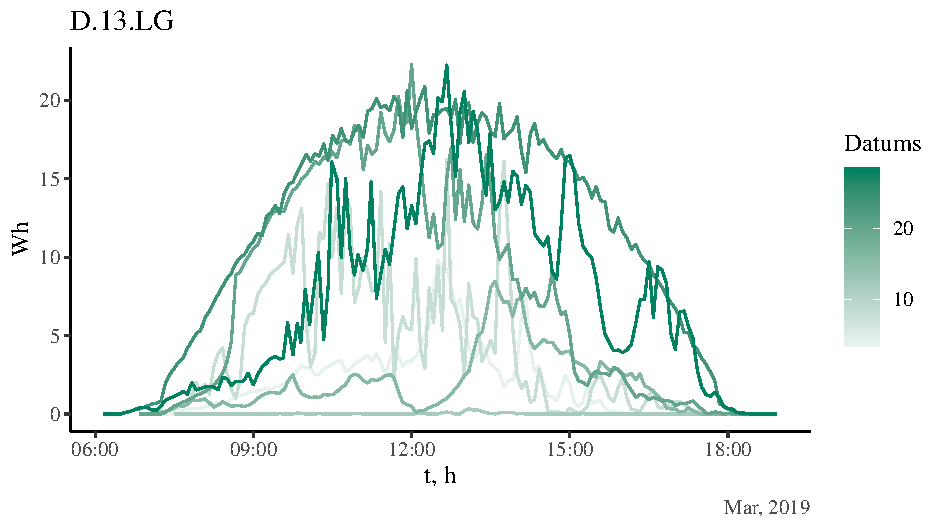
\includegraphics[width=\linewidth]{figures/mar_day/mar_D13LG.pdf}
%     \captionof{figure}{Saražotās enerģijas sadalījuma izmaiņas mēneša dienās saules panelim martā}
% \end{center}
% \begin{center}
%     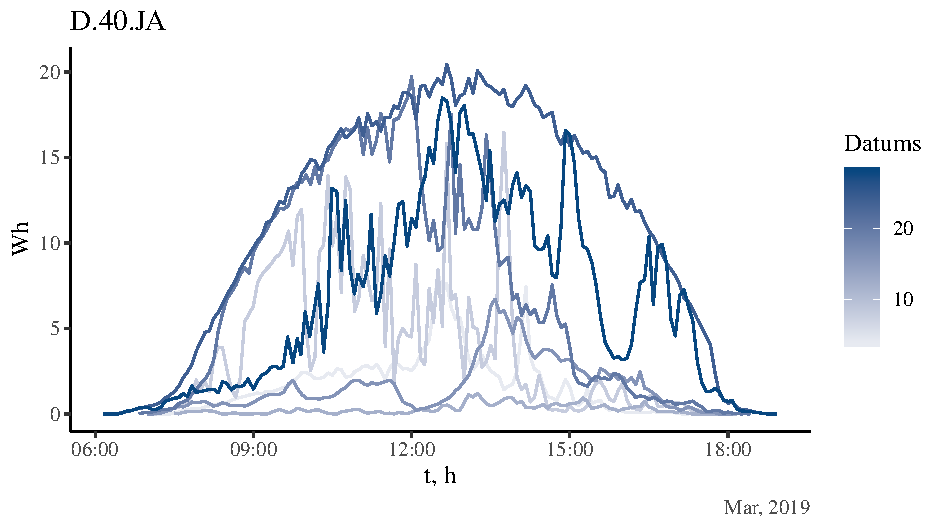
\includegraphics[width=\linewidth]{figures/mar_day/mar_D40JA.pdf}
%     \captionof{figure}{Saražotās enerģijas sadalījuma izmaiņas mēneša dienās saules panelim martā}
% \end{center}
% \begin{center}
%     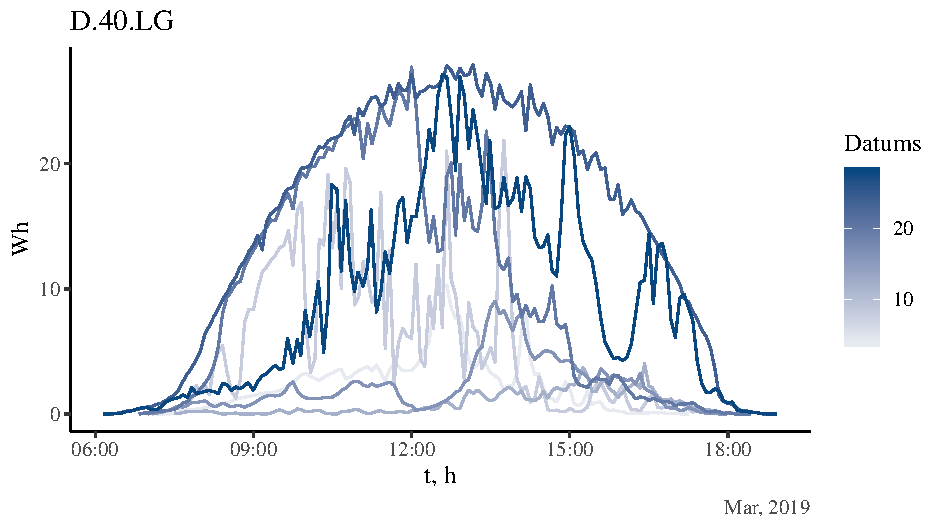
\includegraphics[width=\linewidth]{figures/mar_day/mar_D40LG.pdf}
%     \captionof{figure}{Saražotās enerģijas sadalījuma izmaiņas mēneša dienās saules panelim martā}
% \end{center}
% \begin{center}
%     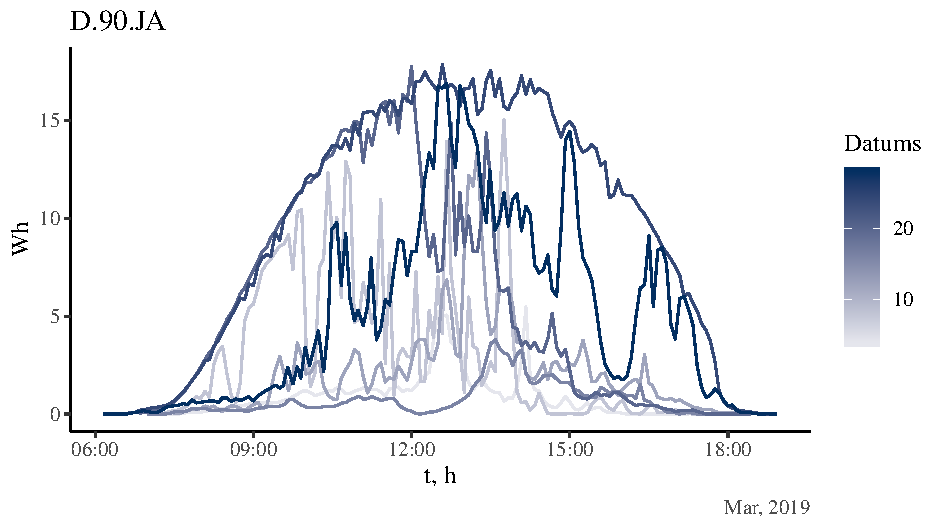
\includegraphics[width=\linewidth]{figures/mar_day/mar_D90JA.pdf}
%     \captionof{figure}{Saražotās enerģijas sadalījuma izmaiņas mēneša dienās saules panelim martā}
% \end{center}
% \begin{center}
%     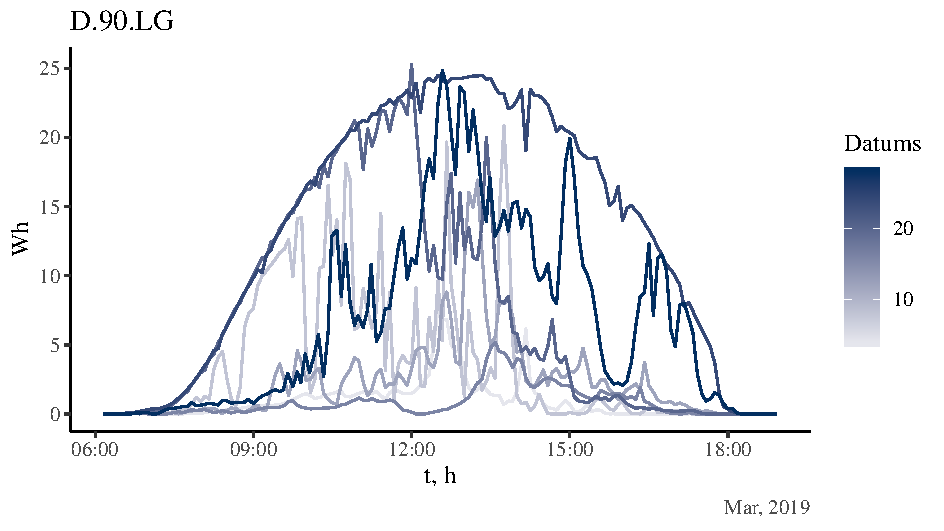
\includegraphics[width=\linewidth]{figures/mar_day/mar_D90LG.pdf}
%     \captionof{figure}{Saražotās enerģijas sadalījuma izmaiņas mēneša dienās saules panelim martā}
% \end{center}
% \begin{center}
%     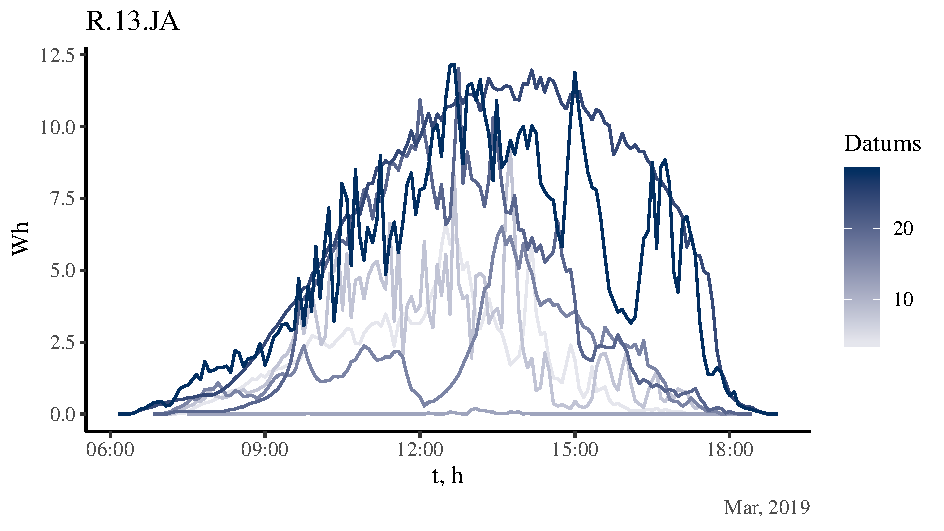
\includegraphics[width=\linewidth]{figures/mar_day/mar_R13JA.pdf}
%     \captionof{figure}{Saražotās enerģijas sadalījuma izmaiņas mēneša dienās saules panelim martā}
% \end{center}
% \begin{center}
%     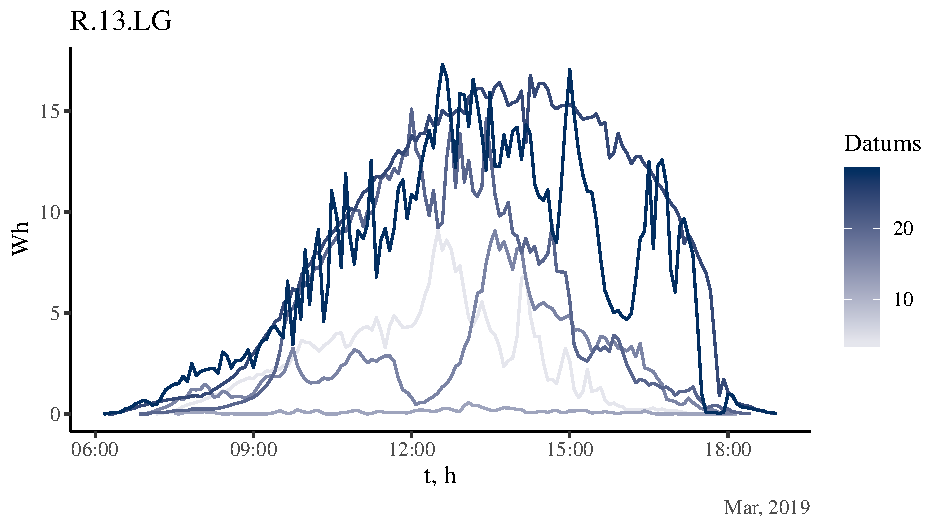
\includegraphics[width=\linewidth]{figures/mar_day/mar_R13LG.pdf}
%     \captionof{figure}{Saražotās enerģijas sadalījuma izmaiņas mēneša dienās saules panelim martā}
% \end{center}
% \begin{center}
%     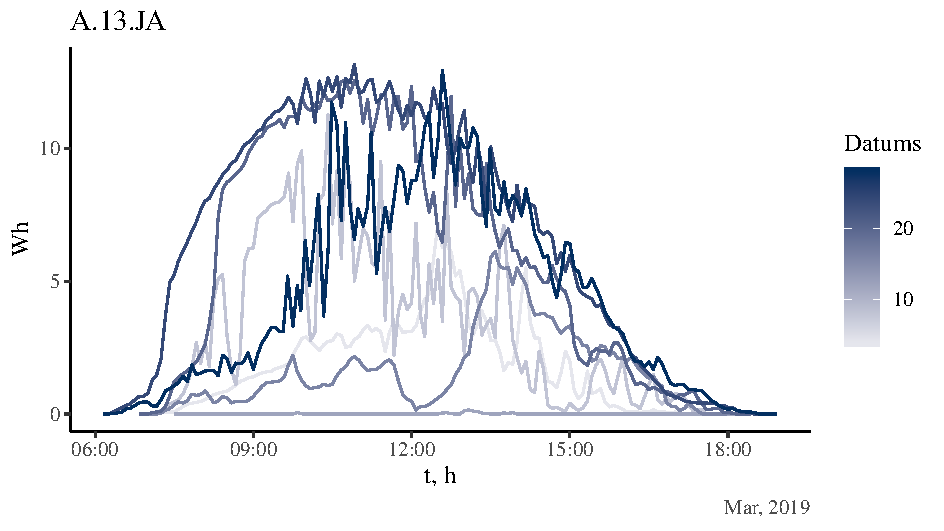
\includegraphics[width=\linewidth]{figures/mar_day/mar_A13JA.pdf}
%     \captionof{figure}{Saražotās enerģijas sadalījuma izmaiņas mēneša dienās saules panelim martā}
% \end{center}
% \begin{center}
%     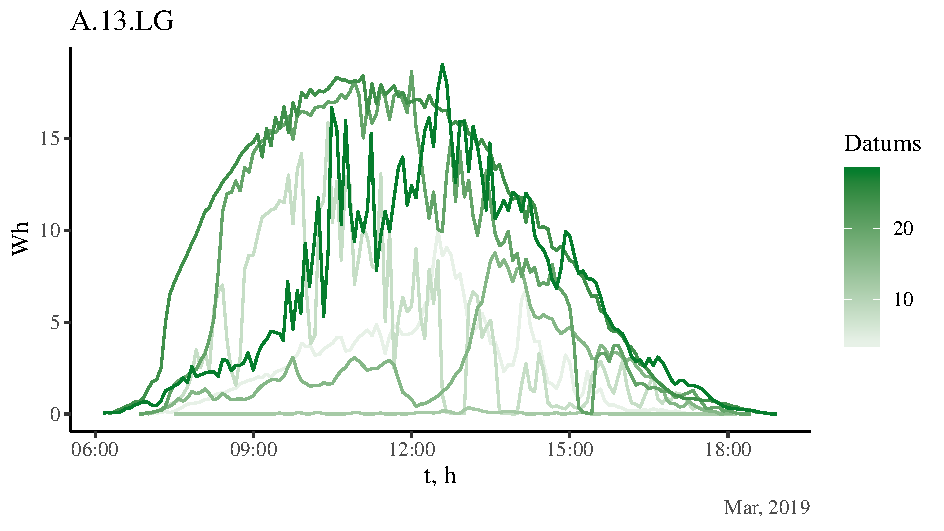
\includegraphics[width=\linewidth]{figures/mar_day/mar_A13LG.pdf}
%     \captionof{figure}{Saražotās enerģijas sadalījuma izmaiņas mēneša dienās saules panelim martā}
% \end{center}